\section{Projektanforderungen} \label{Projektanforderungen}

	Die Thesis basiert auf einem offen definierten Auftrag ohne ein festgelegtes Lastenheft, wodurch die Projektanforderungen entsprechend flexibel gestaltet sind. Um jedoch einen effizienten und zielgerichteten Workflow zu gewährleisten – insbesondere bei einem Projekt dieser Grössenordnung – ist es entscheidend, klare Projektziele zu definieren.
	\\
	Für die Definition der Projektanforderungen wird eine bewährte Methode aus dem System- und Anforderungsmanagement genutzt, bei der «Needs», «Goals» und «Objectives» (NGOs) formuliert werden (Tab. \ref{tab:Projektanforderungen}). Ein «Need» beschreibt in einer einzigen Aussage, welches Problem das System lösen soll, ohne dabei konkrete Lösungen vorzugeben. Die «Goals» legen die Erwartungen an das System fest, die zur Erfüllung des «Needs» beitragen. Darauf aufbauend definieren die «Objectives» spezifische Anforderungen für jedes «Goal». Ein zentraler Aspekt dieser Anforderungen ist, dass sie messbar, quantifizierbar und überprüfbar sein müssen.
	\\
	\\
	Folgende NGO's wurden für die Thesis definiert: 
	
	\begin{table}[h!]
		\centering
		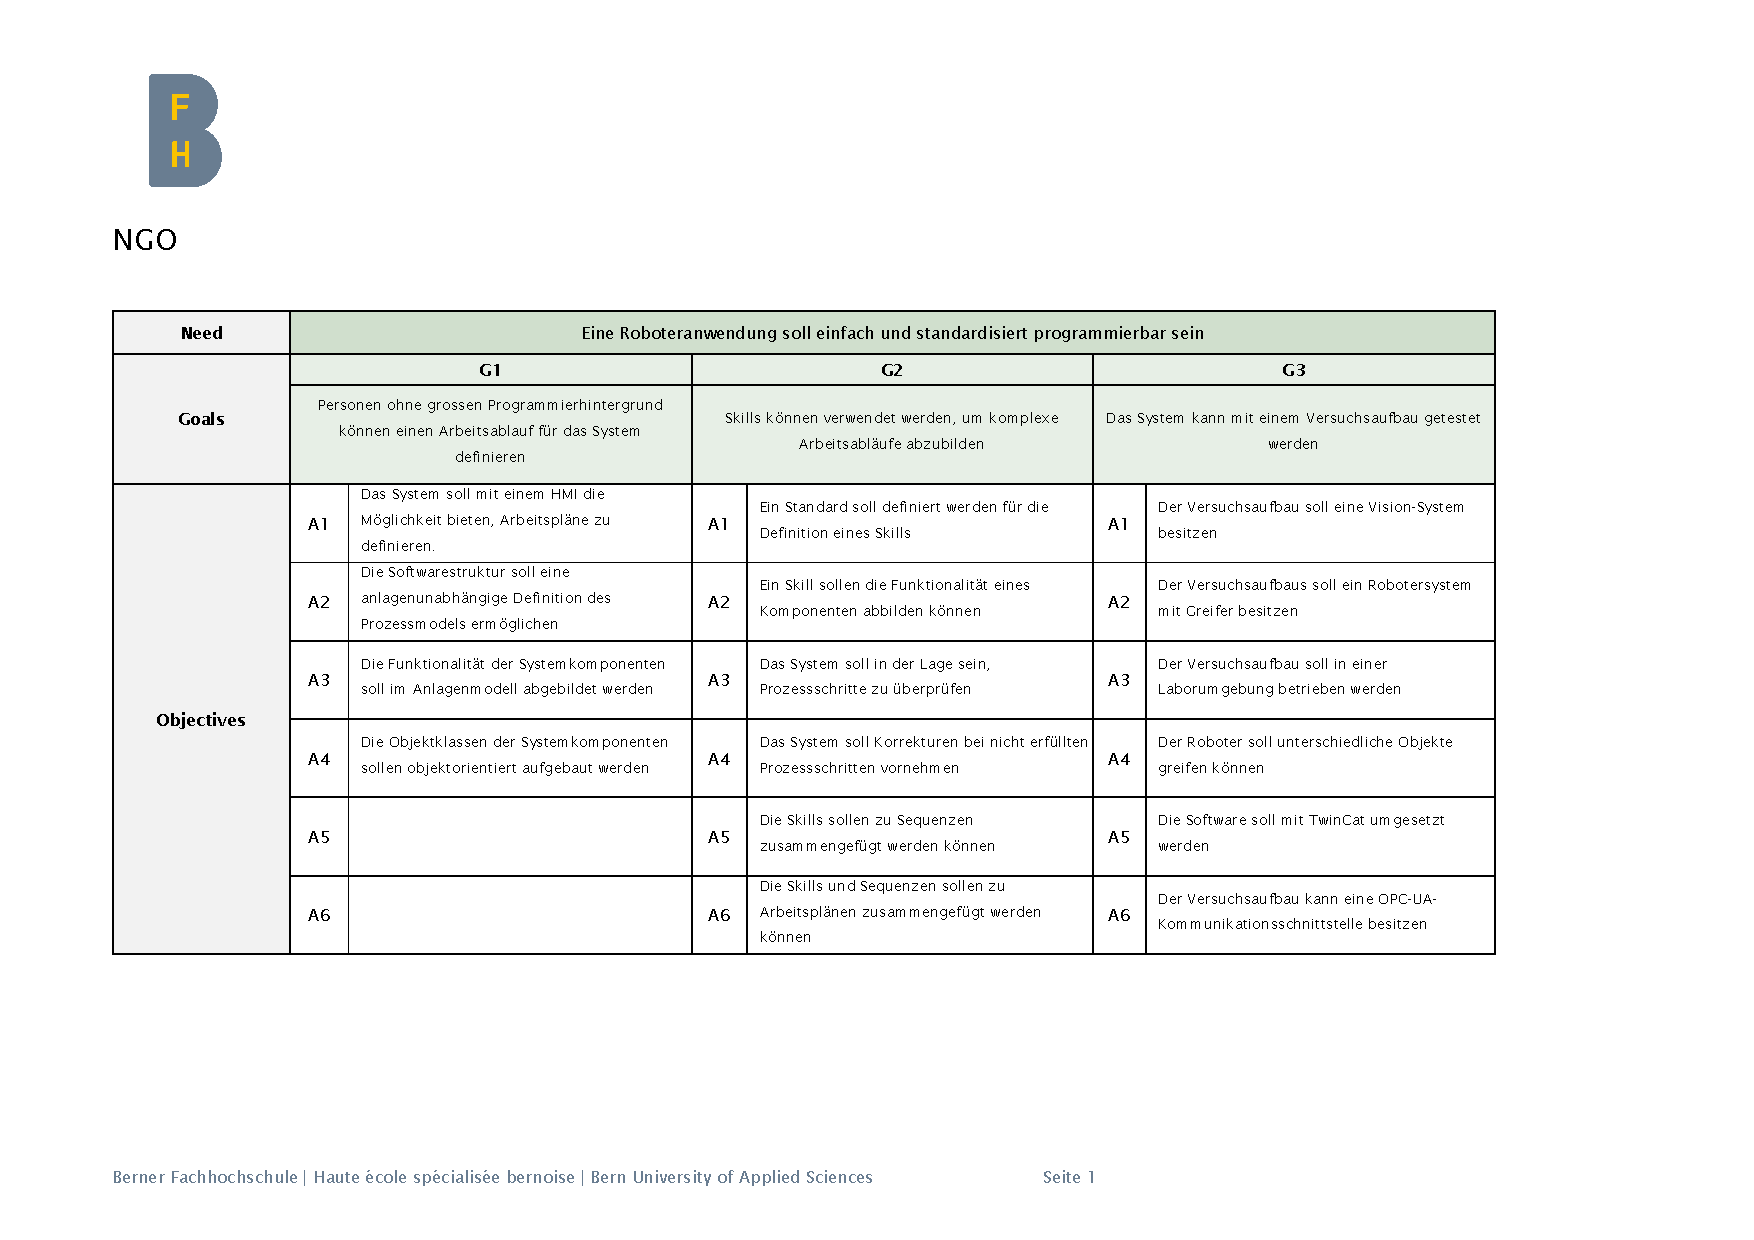
\includegraphics[width=1\textwidth]{02_Einfuehrung_in_Thematik/NGO}
		\caption{Projektanforderungen}
		\label{tab:Projektanforderungen}
	\end{table}
	
	Mit der Definition der Projektanforderungen wird die Analyse-Phase abgeschlossen. Die gewonnen Erkenntnisse werden in einem nächsten Schritt als Grundlage für die Planung der weiteren Phasen verwendet. Am Ende des Projektes werden die definierten Anforderungen mit der umgesetzten Lösung verglichen. 